\section{Intégration du LiDAR sur une plateforme robotique}
\subsection{Integration mécanique}
\tab Il a fallu là aussi réfléchir à la meilleure option compte tenu de notre système. Le robot sur lequel nous posons le LiDAR participe à la Coupe de France de Robotique. Le règlement de la coupe impose à tout participant d'avoir un robot dont la hauteur n'excède pas 35cm. Cependant, ils doivent tous avoir un support de balise de 8cm de haut à une hauteur de 35cm jusqu'à 43cm. Ce support balise doit être opaque et suffisamment gros (cylindre de 70 à 100m de diamètre positionné au centre du robot). Comme nous n'avons aucune assurance sur la taille d'un robot adverse et que c'est l'élément principal si ce n'est le seul que nous voulons détecter, nous ne pouvons essayer de détecter à la hauteur que nous voulons. Nous avons donc fait le choix de mettre le LiDAR à l'intérieur du support balise. En effet, comme nous avons le droit à un trou jusqu'à 2cm de hauteur sur le support de balise, nous pouvons l'intégrer à l'intérieur dans l'espoir de détecter le support balise de l'adversaire. Comme nous sommes certains que tous les robots posséderont un support balise, nous sommes confiants sur la possibilité de détecter l'adversaire.

\begin{figure}[htp]
    \centering
    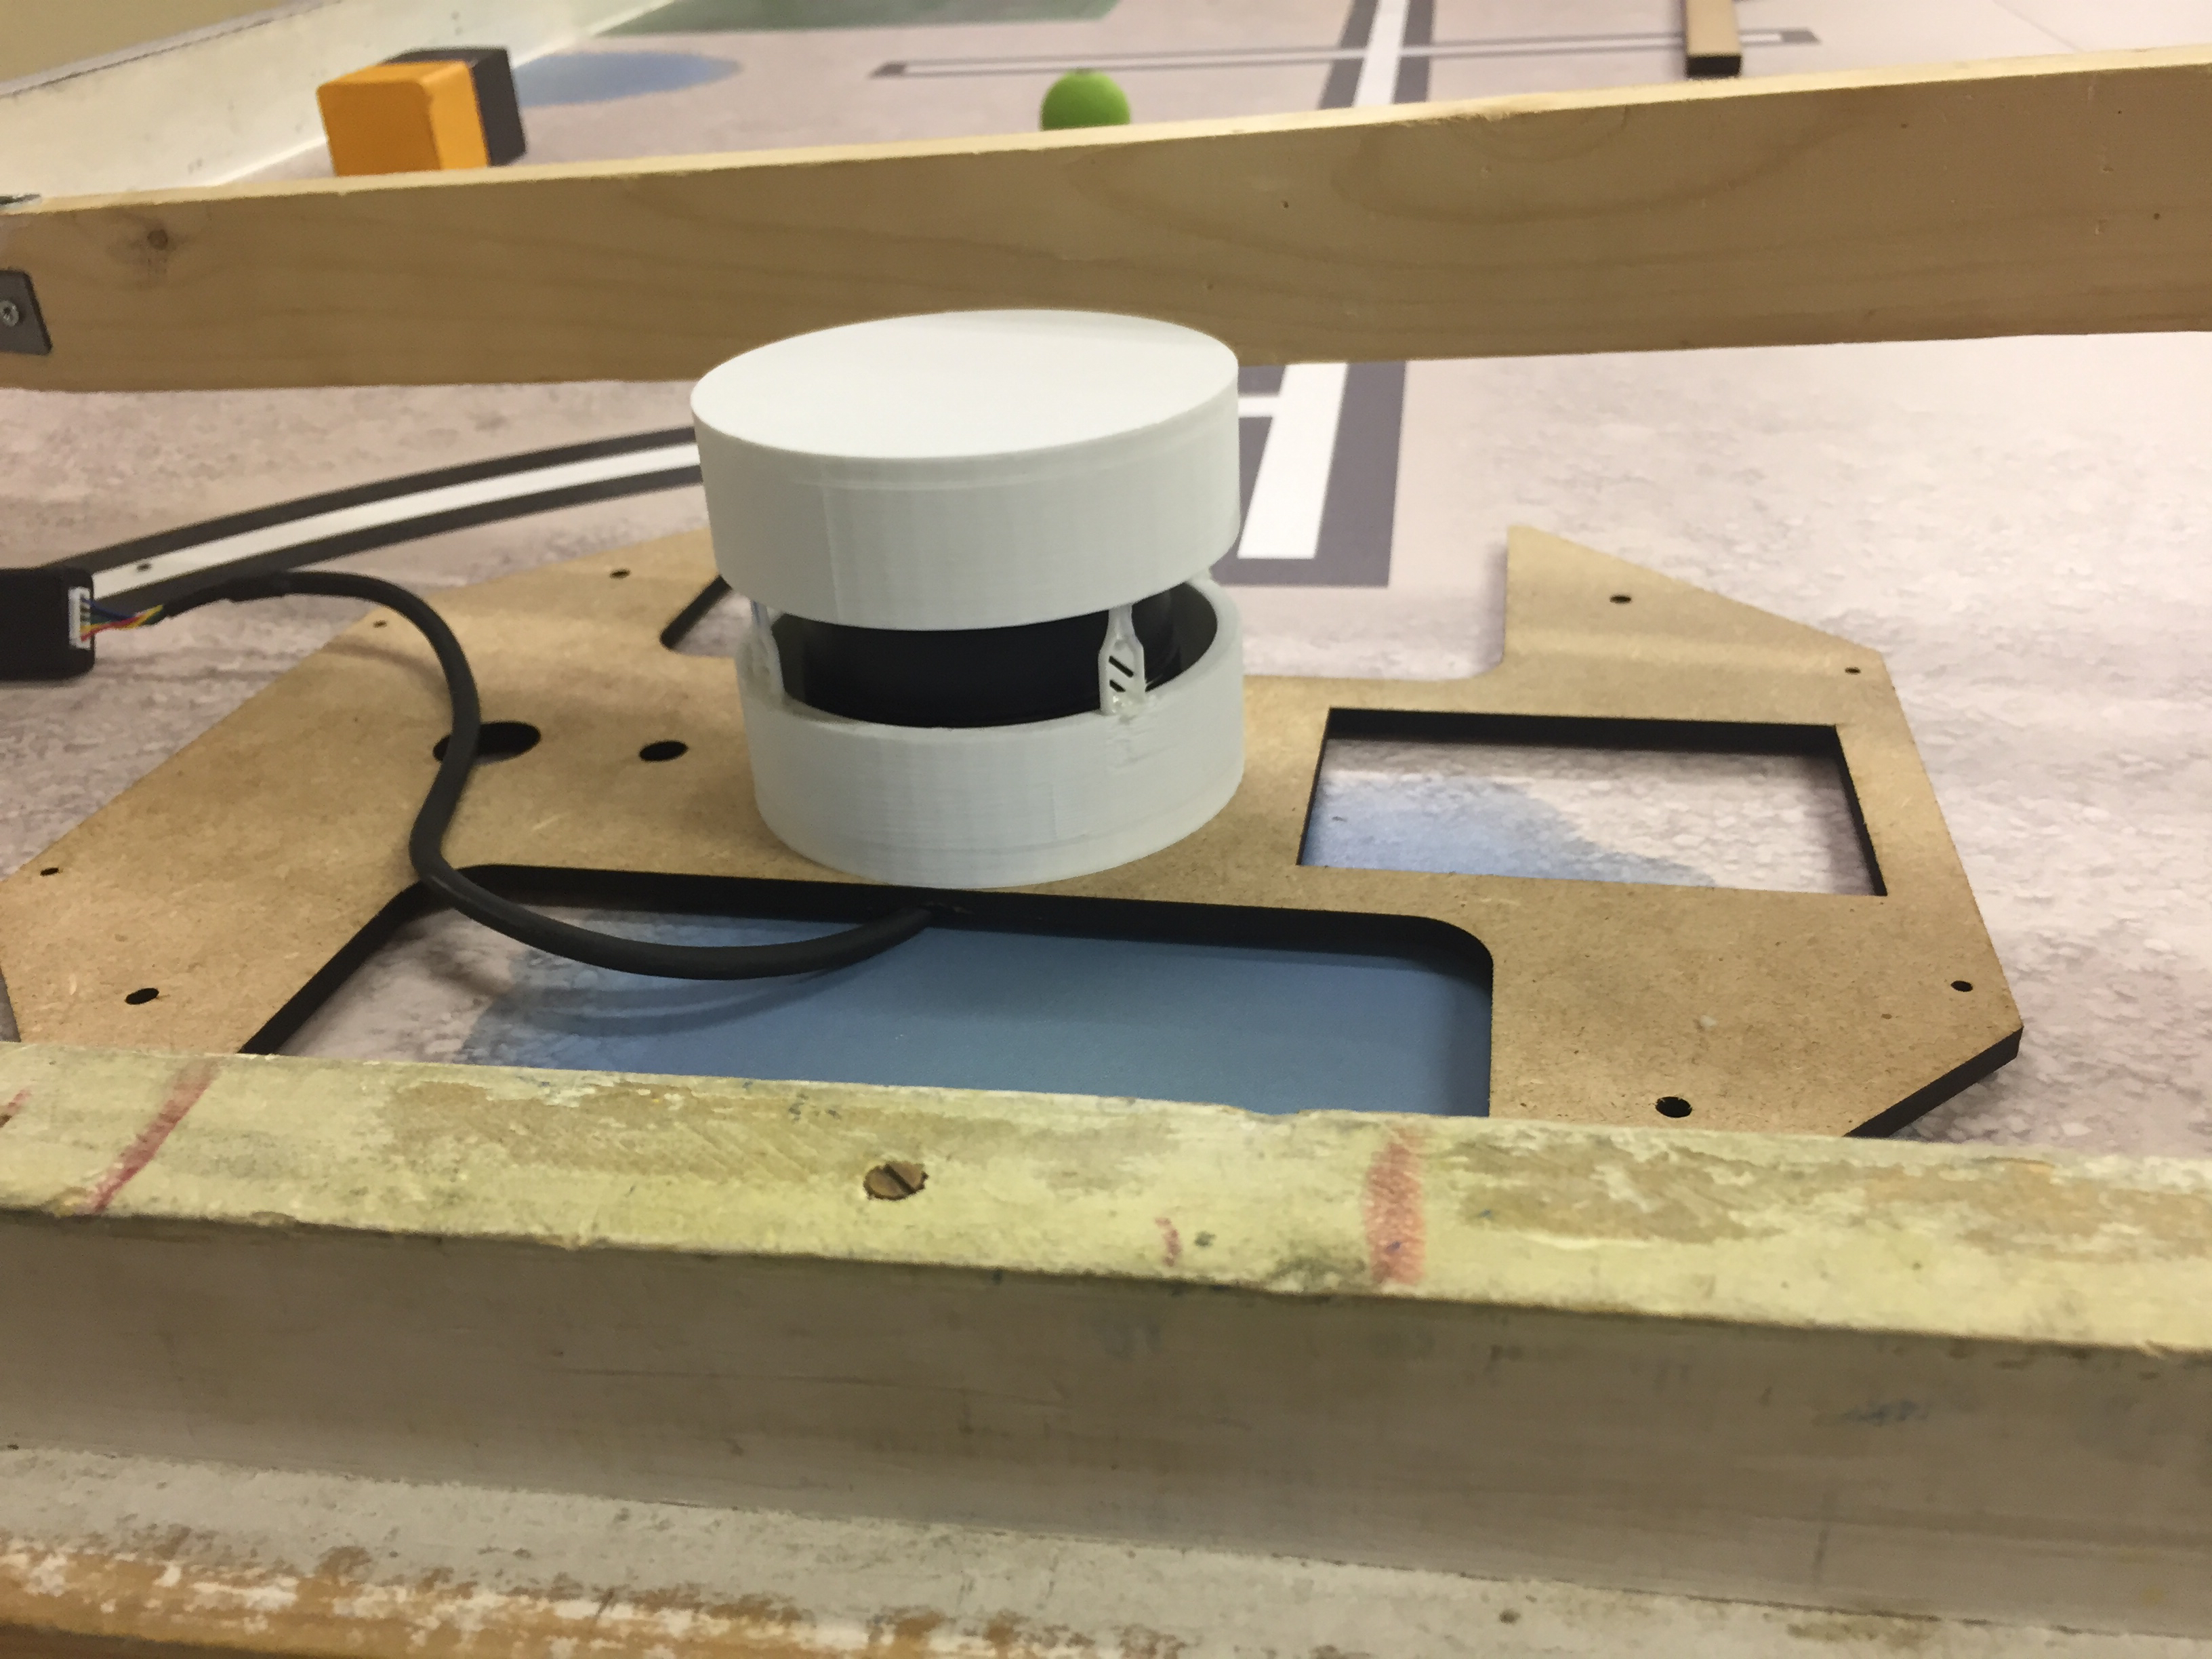
\includegraphics[width=6cm]{images/Integration/integration_robot.jpg}
    \caption{Début du montage sur le robot.}
\end{figure}

\begin{figure}[htp]
    \centering
    \includegraphics[width=6cm]{images/Integration/robot_intech.png}
    \caption{LiDAR en action sur le robot INTech.}
\end{figure}

\subsection{Interfaçage avec le pathfinding}
% probleme RPI => CODE C

\tab L'objectif était de pouvoir envoyer la position des obstacles détectés à un code en Java qui contenait la gestion complète de la stratégie du robot du club de robotique INTech. Ce code implémentait donc notamment un \textit{pathfinding} qui avait vocation à traiter les informations fournies par notre code associé au LiDAR.  

Après discussion, la solution adoptée a été la suivante:
\begin{enumerate}
    \item lancer notre code Python à partir du code Java
    \item créer une \textit{socket} afin d'envoyer le centre de la position de chaque obstacle au code Java
    \item le \textit{pathfinding} peut alors utiliser ces informations pour calculer un nouveau chemin et éviter un potentiel obstacle
\end{enumerate}
\tab L'interfaçage avec le \textit{pathfinding} a été réalisé avec succès, mais a soulevé un nouveau problème : sur le Raspberry Pi la capacité de la série python pour lire les informations envoyées par le LiDAR est trop faible, conduisant à une latence croissante au fur et à mesure que l'on effectue des mesures. Ce problème n'apparaissait pas lors de nos tests sur ordinateur, et il s'est avéré que d'autres personnes ont eu le même problème sur Raspberry Pi, y compris en utilisant des librairies C. Le problème semble donc venir de l'implémentation série sur ARM. Une solution trouvée a été de réécrire un code C à la main, permettant de lire très rapidement depuis le LiDAR, sans utiliser des librairies qui sur Raspberry Pi semblent lire trop lentement pour nos besoins.
%On a pas encore testé sur Raspi le code C... Faudrait chopper Julian demain si vous pouvez et le harceler pour filer son code

\subsection{Résultat final}

\tab Ici on peut voir le robot INTech en pleine esquive pour atteindre les cubes visibles dans le fond de l'image. Ci-contre la vidéo:  \href{https://drive.google.com/open?id=1gUHL_6yfKHhAX55Kx0Wif0i2wZ0wc-EG}{Lien de la vidéo.}\footnote{https://drive.google.com/open?id=1gUHL\_6yfKHhAX55Kx0Wif0i2wZ0wc-EG}

On peut également observer le robot et son LiDAR en plein match lors de la Coupe d'Île de France 2018 :
\href{https://drive.google.com/open?id=1vG5ts-w3lH8zYN6OM3irqqE8x8yshUWw}{Lien de la vidéo.}\footnote{https://drive.google.com/open?id=1vG5ts-w3lH8zYN6OM3irqqE8x8yshUWw}